\chapter{Lec 07 - Adversarial Search II}
\section{Resource Limits}
The minimax algorithm generates the entire game search space, whereas the alpha–beta algorithm allows us to prune large parts of it. However, alpha–beta still has to search all the way to terminal states for at least a portion of the search space. This depth is usually not practical, because moves must be made in a reasonable amount of time (typically a few minutes at most). The solution is to alter minimax or alpha-beta in two ways: replace the utility function by a heuristic \textbf{evaluation function} EVAL, which estimates the position’s utility, and replace the terminal test by a \textbf{cutoff test} that decides when to apply EVAL (e.g. depth limit).

\section{Evaluation functions}
An evaluation function returns an estimate of the expected utility of the game from a given position, just as the heuristic functions return an estimate of the distance to the goal. It should be clear that the performance of a game-playing program depends strongly on the quality of its evaluation function. How exactly do we design good evaluation functions?\newline\newline
First, the evaluation function should order the terminal states in the same way as the true utility function: states that are wins must evaluate better than draws, which in turn must be better than losses. Second, the computation must not take too long. Third, for nonterminal states, the evaluation function should be strongly correlated with the actual chances of winning.

\subsection{Quiescence Search}
\begin{center}
    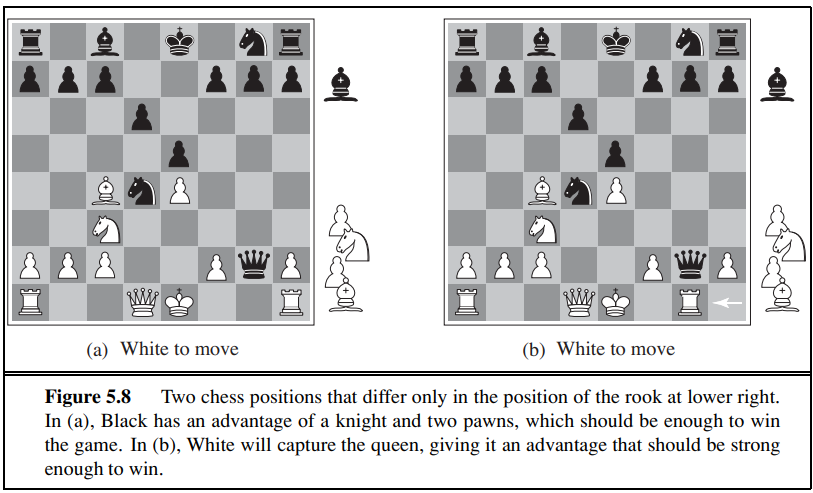
\includegraphics[scale=0.8]{images/quiescence.png}
\end{center}
Suppose the program searches to the depth limit, reaching the position in the figure above, where Black is ahead by a knight and two pawns. If the EVAL function was based only on the number of pieces on the board, it would declare that the state is a probable win by Black. But White’s next move captures Black’s queen with no compensation. Hence, the position is really won for White, but this can be seen only by looking ahead one more ply. Obviously, a more sophisticated cutoff test is needed. The evaluation function should be applied only to positions that are \textbf{quiescent}, that is, unlikely to exhibit wild swings in value in the near future. Non-quiescent positions can be expanded further until quiescent positions are reached.
\newline\newline
The \textbf{horizon effect} is more difficult to eliminate. It arises when the program is facing an opponent’s move that causes serious damage and is ultimately unavoidable, but can be temporarily avoided by delaying tactics. One strategy to mitigate the horizon effect is the \textbf{singular extension}, a move that is “clearly better” than all other moves in a given position. Once discovered anywhere in the tree in the course of a search, this singular move is remembered. When the search reaches the normal depth limit, the algorithm checks to see if the singular extension is a legal move; if it is, the algorithm allows the move to be considered. This makes the tree deeper, but because there will be few singular extensions, it does not add many total nodes to the tree.

\section{Non-deterministic Games}
In real life, many unpredictable external events can put us into unforeseen situations. Many games mirror this unpredictability by including a random element, such as the throwing of dice.\newline\newline
Backgammon is a typical game that combines luck and skill. Dice are rolled at the beginning of a player’s turn to determine the legal moves. Although White knows what his or her own legal moves are, White does not know what Black is going to roll and thus does not know what Black’s legal moves will be. That means White cannot construct a standard game tree of the sort we saw in chess and tic-tac-toe. A game tree in backgammon must include \textbf{chance nodes} in addition to MAX and MIN nodes.
\begin{center}
    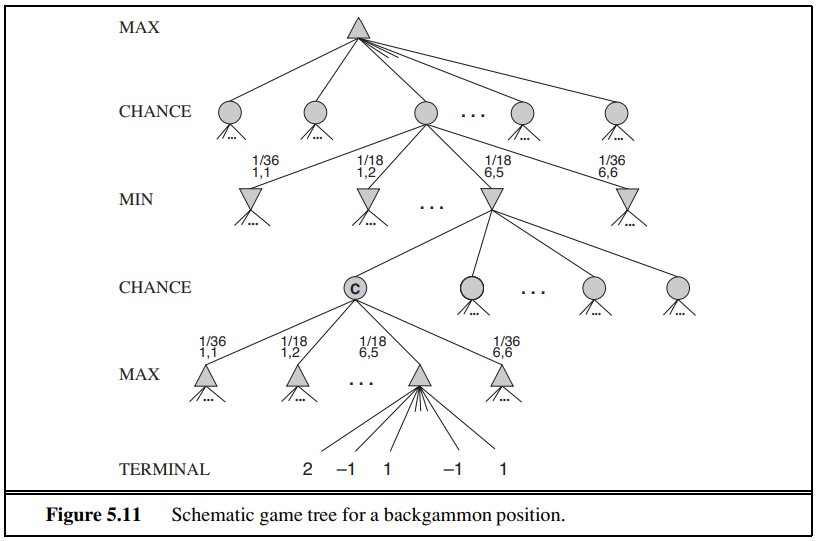
\includegraphics[scale=0.8]{images/chance nodes.png}
\end{center}
The branches leading from each chance node denote the possible dice rolls; each branch is labeled with the roll and its probability. There are 36 ways to roll two dice, each equally likely; but because a 6-5 is the same as a 5-6,
there are only 21 distinct rolls.\newline\newline
The next step is to understand how to make correct decisions. Obviously, we still want to pick the move that leads to the best position. However, positions do not have definite minimax values. Instead, we can only calculate the \textbf{expected value} of a position: the average over all possible outcomes of the chance nodes.\newline\newline
This leads us to generalize the minimax value for deterministic games to an \textbf{expecti-minimax value} for games with chance nodes. Terminal nodes and MAX and MIN nodes (for which the dice roll is known) work exactly the same way as before. For chance nodes we compute the expected value, which is the sum of the value over all outcomes, weighted by the probability of each chance action:
\begin{center}
    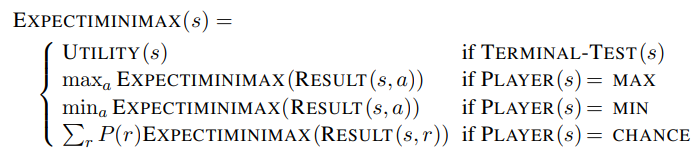
\includegraphics[]{images/expectiminimax.png}
\end{center}
where $r$ represents a possible dice roll (or other chance event).\newline\newline
Note that alpha-beta pruning is still possible for non-deterministic game trees. In fact, for chance nodes, $\alpha$ and $\beta$ are computed by multiplying the value of each MAX and MIN nodes by the respective probability. Stronger pruning can be obtained if possible to bound the leaves values.

\subsection{Evaluation functions for games of chance}
As with minimax, the obvious approximation to make with expectiminimax is to cut the search off at some point and apply an evaluation function to each leaf. One might think that evaluation functions for games such as backgammon should be just like evaluation functions for chess, they just need to give higher scores to better positions. But in fact, the presence of chance nodes means that one has to be more careful about what the evaluation values mean.
\begin{center}
    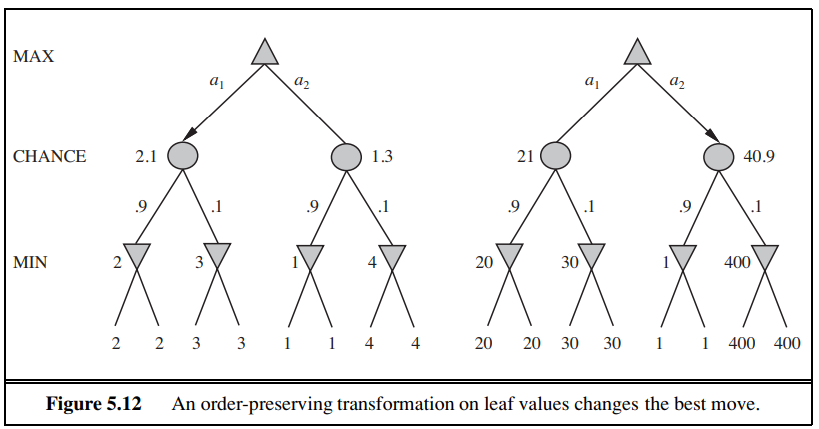
\includegraphics[]{images/eval-stoch-games.png}
\end{center}
With an evaluation function that assigns the values [1, 2,
3, 4] to the leaves, move $a_1$ is best; with values [1, 20, 30, 400], move $a_2$ is best. Hence, the program behaves totally differently if we make a change in the scale of some evaluation values! It turns out that to avoid this sensitivity, the evaluation function must be a positive linear transformation of the probability of winning from a position (or, more generally, of the expected utility of the position).\newline\newline
Because expectiminimax is also considering all the possible dice-roll sequences, it will take $O(b^m n^m)$ where $n$ is the number of distinct rolls. Even if the search depth is limited to some small depth $d$, the extra cost compared with that of minimax makes it unrealistic to consider looking ahead very far in most games of chance.  In backgammon $n$ is 21 and $b$ is usually around 20, but in some situations can be as high as 4000 for dice rolls that are doubles.

\section{Partially Observable Games}
Partially Observable Games are games with hidden information, for example card games, where opponent’s initial cards are unknown.\newline\newline
At first sight, it might seem that these card games are just like dice games: the cards are dealt randomly and determine the moves available to each player, but all the “dice” are rolled at the beginning! Even though this analogy turns out to be incorrect, it suggests an effective algorithm: consider all possible deals of the invisible cards; solve each one as if it were a fully observable game; and then choose the move that has the best outcome averaged over all the deals. Suppose that each deal $s$ occurs with probability $P(s)$; then the move we want is:
\[argmax_a\sum_{s} P(s)\text{MINIMAX(RESULT($s, a$))}\]
Now, in most card games, the number of possible deals is rather large.  Solving even one deal is quite difficult, so solving ten million is out of the question. Instead, we resort to a Monte Carlo approximation: instead of adding up all the deals, we take a random sample of $N$ deals, where the probability of deal $s$ appearing in the sample is proportional to $P(s)$:
\[argmax_a \frac{1}{N} \sum_{i=1}^N \text{MINIMAX(RESULT($s_i, a$))}\]
